% 24th, Jan, 2001 Ver.1     Tatsuya Okabe
%                 Ver.2
%                 Ver.3
%                 Ver.4
%                 Ver.5
%
%---------------------------------------------------------------------------%
% Made by Tatsuya Okabe ( HONDA R&D Europe ( Deutschland ) GmbH )           %
% Checked by Bernhard Sendhoff ( HONDA R&D Europe ( Deutschland ) GmbH )    %
%---------------------------------------------------------------------------%
% Array < Class T >

\noindent
In this class several functions were defined to allow the following
operations on arrays :

\vspace*{10mm}

\begin{enumerate}
\item get (a) value(s) of the array
\item append row(s)
\item append column(s)
\item remove row(s)
\item remove column(s)
\item copy a part of the array
\end{enumerate}

\vspace*{10mm}

\noindent
Additionally, the contents of the array can be rearranged and the
transpose can be calculated.

\vspace*{10mm}

\section{Internal Variables}

\begin{itemize}
\item T* e - The data of array.
\item (arraybase) unsigned* d - The pointer to the dimension vector.
\item (arraybase) unsigned nd - The number of dimensions.
\item (arraybase) unsigned ne - The number of elements
\item (arraybase) bool stat - The flag which signals whether object is a static ref.
\end{itemize}

%********************
\index{*e (Variable)}
\index{*d (Variable)}
\index{nd (Variable)}
\index{ne (Variable)}
\index{stat (Variable)}
%********************

\clearpage

\section{Public Methods}

\subsection{Constructors}

%---------------------------------------------------------------------------%
% 001
\index{array!( )}
\setNormalInstance
\printEmptyMethodReturn
{}
{array}
{The default constructor. Generates empty array.}
{None.}
\setCorrectWidthThree{4pt}
%---------------------------------------------------------------------------%

%---------------------------------------------------------------------------%
% 002
\index{array!( unsigned i )} 
\setNormalInstance
\printMethodWithOneParam
{explicit}
{array}
{unsigned}
{i}
{The size of an one-dimensional array.}
{The copy constructor. Generates new array with one-dimension ``{\em i}''.}
{None.}
{None.}
%---------------------------------------------------------------------------%

%---------------------------------------------------------------------------%
% 003
\index{array!( unsigned i, unsigned j )}
\setNormalInstance
\setCorrectWidthThree{8pt}
\setParamOne{i}{unsigned}{The size of an one-dimensional array.} 
\setParamTwo{j}{unsigned}{The size of a two-dimensional array.}
\printMethodWithParamsSaved
{}
{None.}
{array}
{The copy constructor. Generates new array with two-dimension ``{\em i
$\times$ j}''.}
{None.}
\setCorrectWidthThree{4pt}
%---------------------------------------------------------------------------%

%---------------------------------------------------------------------------%
% 004
\index{array!( unsigned i, unsigned j, unsigned k )}
\setNormalInstance
\setCorrectWidthThree{8pt}
\setParamOne{i}{unsigned}{The size of an one-dimensional array.} 
\setParamTwo{j}{unsigned}{The size of a two-dimensional array.}
\setParamThree{k}{unsigned}{The size of a three-dimensional array.}
\printMethodWithParamsSaved
{}
{None.}
{array}
{The copy constructor. Generates new array with three-dimension ``{\em
i $\times$ j $\times$ k}''.}
{None.}
\setCorrectWidthThree{4pt}
%---------------------------------------------------------------------------%

\clearpage

%---------------------------------------------------------------------------%
% 005
\index{array!( std::vector$<$ T $>$\& v )} 
\setNormalInstance
\printMethodWithOneParam
{}
{array}
{std::vector$<$ T $>$\&}
{v}
{The vector which was set dimensions.}
{The copy constructor. Generates new array from the vector {\em v}.}
{None.}
{None.}
%---------------------------------------------------------------------------%

%---------------------------------------------------------------------------%
% 006
\index{array!( array$<$ T $>$\& v, bool )}
\setNormalInstance
\setCorrectWidthThree{8pt}
\setParamOne{v}{array$<$ T $>$\&}{The array you want copy.} 
\setParamTwo{}{bool}{The dummy value.}
\printMethodWithParamsSaved
{}
{None.}
{array}
{The copy constructor. Generates new array by copying the array ``{\em v}'' and
sets the array ``{\em v}'' as a reference.}
{None.}
\setCorrectWidthThree{4pt}
%---------------------------------------------------------------------------%

%---------------------------------------------------------------------------%
% 007
\index{array!( const array$<$ T $>$\& v)} 
\setNormalInstance
\printMethodWithOneParam
{}
{array}
{const array$<$ T $>$\&}
{v}
{The array you want to copy.}
{The copy construtor. Generates new array by copying the array ``{\em v}'' }
{None.}
{None.}
%---------------------------------------------------------------------------%

\vspace*{10mm}

\subsection{Destructor}

%---------------------------------------------------------------------------%
% 008
\index{$\sim$array!()} 
\setNormalInstance
\printEmptyMethodReturnSpecial
{}
{$\sim$array}
{The distructor. Destroys the current array {\em this}.}
{None.}
{The destructor should not be called directly.}
%---------------------------------------------------------------------------%

\clearpage

\subsection{Operators}

%---------------------------------------------------------------------------%
% 009
\index{operator( )!( )} 
\setNormalInstance
\printEmptyMethodReturn
{T\&}
{operator( )}
{Returns the value {\em e[0]} ( The first value of this array ) if the
number of dimensions is {\em 0} and the number of elements is {\em 1}.}
{The velue of {\em e[0]} ( The first value of this array ).}
%---------------------------------------------------------------------------%

%---------------------------------------------------------------------------%
% 010
\index{operator( )!( )} 
\setConstInstance
\printEmptyMethodReturn
{T\&}
{operator( )}
{Returns the value {\em e[0]} as a constant, if the number of
dimensions is {\em 0} and the number of elements is {\em 1}}
{The value of {\em e[0]} ( The first value of this array ).}
%---------------------------------------------------------------------------%

%---------------------------------------------------------------------------%
% 011
\index{operator( )!( unsigned i )} 
\setNormalInstance
\printMethodWithOneParam
{T\&}
{operator( )}
{unsigned}
{i}
{The number in 1D whose value you want to know.}
{Returns the value {\em e[i]}, if the number of dimensions is {\em 1}
and {\em i} $\le$ the number of elements.}
{The value {\em e[i]}.}
{None.}
%---------------------------------------------------------------------------%

%---------------------------------------------------------------------------%
% 012
\index{operator( )!( unsigned i )} 
\setConstInstance
\printMethodWithOneParam
{T\&}
{operator( )}
{unsigned}
{i}
{The number in 1D whose value you want to know.}
{Returns the value {\em e[i]} as a constant, if the number of
dimensions is {\em 1} and {\em i} $\le$ the number of elements.}
{The value {\em e[i]}.}
{None.}
%---------------------------------------------------------------------------%

\clearpage

%---------------------------------------------------------------------------%
% 013
\index{operator( )!( unsigned i, unsigned j )}
\setNormalInstance
\setCorrectWidthThree{8pt}
\setParamOne{i}{unsigned}{The number in 1D whose you want to know.} 
\setParamTwo{j}{unsigned}{The number in 2D whose you want to know.}
\printMethodWithParamsSaved
{T\&}
{The value of {\em e(i,j)} ( {\em e(d[1]*i+j)} ).}
{operator( )}
{Returns the value {\em e(i,j)}, if the number of dimensions is {\em
2}, {\em i} $\le$ the number of 1-dimensional elements and {\em j} $\le$ the
number of 2-dimensional elements.}
{The value {\em e(i,j)}.}
\setCorrectWidthThree{4pt}
%---------------------------------------------------------------------------%

%---------------------------------------------------------------------------%
% 014
\index{operator( )!( unsigned i, unsigned j )}
\setConstInstance
\setCorrectWidthThree{8pt}
\setParamOne{i}{unsigned}{The number in 1D whose you want to know.} 
\setParamTwo{j}{unsigned}{The number in 2D whose you want to know.}
\printMethodWithParamsSaved
{T\&}
{The value of {\em e(i,j)} ( {\em e(d[1]*i+j)} ).}
{operator( )}
{Returns the value {\em e(i,j)} as a constant, if the number of dimensions is
{\em 2}, {\em i} $\le$ the number of 1-dimensional elements and {\em j} $\le$ the number of 2-dimensional elements.}
{The value {\em e(i,j)}.}
\setCorrectWidthThree{4pt}
%---------------------------------------------------------------------------%

%---------------------------------------------------------------------------%
% 015
\index{operator( )!( unsigned i, unsigned j, unsigned k )}
\setNormalInstance
\setCorrectWidthThree{8pt}
\setParamOne{i}{unsigned}{The number in 1D whose value you want to know.} 
\setParamTwo{j}{unsigned}{The number in 2D whose value you want to konw.}
\setParamThree{k}{unsigned}{The number in 3D whose value you want to know.}
\printMethodWithParamsSaved
{T\&}
{The value of {\em e(i,j,k)} ( {\em e(d[2]*d[1]*i+d[2]*j+k )} ).}
{operator( )}
{Returns the value {\em e(i,j,k)}, if the number of dimensions is {\em
3}, {\em i} $\le$
the number of 1-dimensional elements, {\em j} $\le$ the
number of 2-dimensional elements and {\em k} $\le$ the number of
3-dimensional elements.}
{The value {\em e(i,j,k)}.}
\setCorrectWidthThree{4pt}
%---------------------------------------------------------------------------%

\clearpage

%---------------------------------------------------------------------------%
% 016
\index{operator( )!( unsigned i, unsigned j, unsigned k )}
\setConstInstance
\setCorrectWidthThree{8pt}
\setParamOne{i}{unsigned}{The number in 1D whose value you want to know.} 
\setParamTwo{j}{unsigned}{The number in 2D whose value you want to know.}
\setParamThree{k}{unsigned}{The number in 3D whose value you want to know.}
\printMethodWithParamsSaved
{T\&}
{The value of {\em e(i,j,k)} ( {\em e(d[2]*d[1]*i+d[2]*j+k )} ).}
{operator( )}
{Returns the value {\em e(i,j,k)} as a constant, if the number of
dimensions is {\em 3}, {\em i} $\le$
the number of 1-dimensional elements, {\em j} $\le$ the
number of 2-dimensional elements and {\em k} $\le$ the number of
3-dimensional elements.}
{The value {\em e(i,j,k)}.}
\setCorrectWidthThree{4pt}
%---------------------------------------------------------------------------%

%---------------------------------------------------------------------------%
% 017
\index{operator( )!( const std::vector$<$ unsigned $>$\& i )} 
\setNormalInstance
\printMethodWithOneParam
{T\&}
{operator( )}
{const std::vector$<$ unsigned $>$\&}
{i}
{The vector which indicates the position of the array, e.g. {\em (i)} : 1D,
{\em (i,j)} : 2D or {\em (i,j,k)} : 3D. Instead of each integer, the
vector ``{\em i}'' is used.}
{Returns the value {\em e(m)}.}
{The value {\em e(i)}.}
{None.}
%---------------------------------------------------------------------------%

%---------------------------------------------------------------------------%
% 018
\index{operator( )!( const std::vector$<$ unsigned $>$\& i )} 
\setConstInstance
\printMethodWithOneParam
{T\&}
{operator( )}
{const std::vector$<$ unsigned $>$\&}
{i}
{The vector which indicates the position of the array, e.g. {\em (i)} : 1D,
{\em (i,j)} : 2D or {\em (i,j,k)} : 3D. Instead of each integer, the
vector ``{\em i}'' is used.}
{Returns the value {\em e(m)} as a constant.}
{The value {\em e(m)}.}
{None.}
%---------------------------------------------------------------------------%

%---------------------------------------------------------------------------%
% 019
%\index{} 
%\setNormalInstance
%\printMethodWithOneParam
%{array\_reference$<$ T $>$}
%{operator[ ]}
%{unsigned}
%{i}
%{}
%{}
%{}
%{The corresponding codes are commented out.}
%---------------------------------------------------------------------------%

%---------------------------------------------------------------------------%
% 020
%\index{} 
%\setConstInstance
%\printMethodWithOneParam
%{array\_reference$<$ T $>$}
%{operator[ ]}
%{unsigned}
%{i}
%{}
%{}
%{}
%{The corresponding codes are commented out.}
%---------------------------------------------------------------------------%

%---------------------------------------------------------------------------%
% 021
\index{operator =!( const T\& v )} 
\setNormalInstance
\printMethodWithOneParam
{array$<$ T $>$\&}
{operator =}
{const T\&}
{v}
{The normal array in \cpp.}
{Changes the ``{\em v}'' into the array in this class {\em array}.}
{The array ``{\em this}''.}
{None.}
%---------------------------------------------------------------------------%

\clearpage

%---------------------------------------------------------------------------%
% 022
\index{operator =!( const std::vector$<$ T $>$\& v} 
\setNormalInstance
\printMethodWithOneParam
{array$<$ T $>$\&}
{operator=}
{const std::vector$<$ T $>$\&}
{v}
{The vector.}
{Changes the ``{\em v}'' into the array in this class {\em array}.}
{The array ``{\em this}''.}
{None.}
%---------------------------------------------------------------------------%

%---------------------------------------------------------------------------%
% 023
\index{operator =!( const array$<$ T $>$\& v )} 
\setNormalInstance
\printMethodWithOneParam
{array$<$ T $>$\&}
{operator=}
{const array$<$ T $>$\&}
{v}
{The array ``{\em v}''.}
{Handles the special case of assigning an empty array in order to
avoid uninitialized memory read (purify).}
{The array from ``{\em this}''.}
{None.}
%---------------------------------------------------------------------------%

\clearpage

\subsection{Methods of getting the data in the array.}

%---------------------------------------------------------------------------%
% 024
\index{elem!( unsigned i )} 
\setNormalInstance
\printMethodWithOneParam
{T\&}
{elem}
{unsigned}
{i}
{The number of data you want to get.}
{Returns the value of ``{\em i}''th data in the array.}
{The value of ``{\em i}''th data in the array ``{\em e[i]}''.}
{None.}
%---------------------------------------------------------------------------%

%---------------------------------------------------------------------------%
% 025
\index{elem!( unsigned i )} 
\setConstInstance
\printMethodWithOneParam
{T\&}
{elem}
{unsigned}
{i}
{The number of data you want to get.}
{Returns the value of ``{\em i}''th data in the array as a constant.}
{The value of ``{\em i}''th data in the array ``{\em e[i]}''.}
{None.}
%---------------------------------------------------------------------------%

%---------------------------------------------------------------------------%
% 026
\index{elemvec!( )} 
\setNormalInstance
\printEmptyMethodReturn
{T*}
{elemvec}
{Returns the vector ``{\em e}''.}
{The vector ``{\em e}''.}
%---------------------------------------------------------------------------%

%---------------------------------------------------------------------------%
% 026a
\index{elemvec!( )} 
\setConstInstance
\printEmptyMethodReturn
{T*}
{elemvec}
{Returns the vector ``{\em e}'' as a constant.}
{The vector ``{\em e}''.}
%---------------------------------------------------------------------------%

%---------------------------------------------------------------------------%
% 067
\index{dimarr!( )} 
\setConstInstance
\printEmptyMethodReturn
{array$<$ unsigned $>$}
{dimarr}
{Returns the dimension array ( vector ) ``{\em d}''.}
{The dimension array ``{\em d}''.}
%---------------------------------------------------------------------------%

\clearpage

\subsection{Structure Changing Methods}

\vspace*{5mm}

\noindent
Append.

%---------------------------------------------------------------------------%
% 027
\index{append\_elem!( const T\& w )} 
\setNormalInstance
\printMethodWithOneParam
{array$<$ T $>$\&}
{append\_elem}
{const T\&}
{w}
{The data you want to append in this array.}
{Appends the data.}
{The array ``{\em this}''.}
{This function needs the empty or 1-Dimensional array.}
%---------------------------------------------------------------------------%

%---------------------------------------------------------------------------%
% 028
\index{append\_elems!( const array$<$ T $>$\& w )} 
\setNormalInstance
\printMethodWithOneParam
{array$<$ T $>$\&}
{append\_elems}
{const array$<$ T $>$\&}
{w}
{The array you want to append in this array.}
{Appends the array ( 1-Dimension ).}
{The array ``{\em this}''.}
{This functioin needs the empty or 1-Dimensional array.}
%---------------------------------------------------------------------------%

%---------------------------------------------------------------------------%
% 029
\index{append\_rows!( const array$<$ T $>$\& y} 
\setNormalInstance
\printMethodWithOneParam
{array$<$ T $>$\&}
{append\_rows}
{const array$<$ T $>$\&}
{y}
{The array you want to append after the last row of this array.}
{Appends the array ``{\em y}'' after the last row.}
{The array {\em this}.}
{This function needs the empty array or the same dimensional array or
-1 dimensional array of {\em y}.}
%---------------------------------------------------------------------------%

%---------------------------------------------------------------------------%
% 040
\index{append\_cols!( const array$<$ T $>$\& y )} 
\setConstInstance
\printMethodWithOneParam
{array$<$ T $>$\&}
{append\_cols}
{const array$<$ T $>$\&}
{y}
{The array you want to append after the last column of this array.}
{Appends the array ``{\em y}'' after the last column.}
{The array ( result ).}
{This function needs that this array is empty or the dimension of this
array is equal to ``{\em y}''.}
%---------------------------------------------------------------------------%

\clearpage

\noindent
Remove.

%---------------------------------------------------------------------------%
% 030
\index{remove\_row!( unsigned i )} 
\setNormalInstance
\printMethodWithOneParam
{array$<$ T $>$\&}
{remove\_row}
{unsigned}
{i}
{The number of row you want to remove. The number starts from {\em 0}.}
{Removes one row from the array.}
{The array ``{\em this}''.}
{This function needs that the dimension of this array is larger than
{\em 0} and ``{\em i}'' is less than or equal to ``{\em d[0]}''.}
%---------------------------------------------------------------------------%

%---------------------------------------------------------------------------%
% 031
\index{remove\_col!( unsigned k )} 
\setConstInstance
\printMethodWithOneParam
{array$<$ T $>$\&}
{remove\_col}
{unsigned}
{k}
{The number of column you want to remove. The number starts from {\em 0}.}
{Removes one column form the array.}
{The array ( result ).}
{This function needs that the dimension of this array is larger than
{\em 0}
and ``{\em i}'' is less than ``{\em dim( ndim( )-1 )}''.}
%---------------------------------------------------------------------------%

%---------------------------------------------------------------------------%
% 032
\index{remove\_cols!( const array$<$ unsigned $>$ idx )} 
\setConstInstance
\printMethodWithOneParam
{array$<$ T $>$}
{remove\_cols}
{const array$<$ unsigned $>$}
{idx}
{The array which has the numbers of columns you want to remove.}
{Removes columns from the array.}
{The array ( result ).}
{None.}
%---------------------------------------------------------------------------%

%---------------------------------------------------------------------------%
% 033
\index{remove\_cols!( unsigned i, unsigned j )}
\setConstInstance
\setCorrectWidthThree{8pt}
\setParamOne{i}{unsigned}{The number of column you want to remove.} 
\setParamTwo{j}{unsigned}{The number of column you want to remove.}
\printMethodWithParamsSaved
{array$<$ T $>$}
{The array ( result ).}
{remove\_cols}
{Removes two columns ``{\em i}'' and ``{\em j}'' from the array.}
{None.}
\setCorrectWidthThree{4pt}
%---------------------------------------------------------------------------%

\clearpage

%---------------------------------------------------------------------------%
% 034
\index{remove\_cols!( unsigned i, unsigned j, unsigned k)}
\setConstInstance
\setCorrectWidthThree{8pt}
\setParamOne{i}{unsigned}{The number of column you want to remove.} 
\setParamTwo{j}{unsigned}{The number of column you want to remove.}
\setParamThree{k}{unsigned}{The number of column you want to remove.}
\printMethodWithParamsSaved
{array$<$ T $>$}
{The array ( result ).}
{remove\_cols}
{Removes three columns ``{\em i}'', ``{\em j}'' and ``{\em k}'' from the array.}
{None.}
\setCorrectWidthThree{4pt}
%---------------------------------------------------------------------------%

\vspace*{-3mm}

%---------------------------------------------------------------------------%
% 035
\index{remove\_cols!( unsigned i, unsigned j, unsigned k, unsinged l )}
\setConstInstance
\setCorrectWidthThree{8pt}
\setParamOne{i}{unsigned}{The number of column you want to remove.} 
\setParamTwo{j}{unsigned}{The number of column you want to remove.}
\setParamThree{k}{unsigned}{The number of column you want to remove.}
\setParamFour{l}{unsigned}{The number of column you want to remove.}
\printMethodWithParamsSaved
{array$<$ T $>$}
{The array ( result ).}
{remove\_cols}
{Removes four columns ``{\em i}'', ``{\em j}'', ``{\em k}'' and ``{\em
l}'' from the array.}
{None.}
\setCorrectWidthThree{4pt}
%---------------------------------------------------------------------------%

\vspace*{-3mm}

%---------------------------------------------------------------------------%
% 036
\index{remove\_cols!( unsigned i, unsigned j, unsigned k, unsinged l,
unsigned m )}
\setConstInstance
\setCorrectWidthThree{8pt}
\setParamOne{i}{unsigned}{The number of column you want to remove.} 
\setParamTwo{j}{unsigned}{The number of column you want to remove.}
\setParamThree{k}{unsigned}{The number of column you want to remove.}
\setParamFour{l}{unsigned}{The number of column you want to remove.}
\setParamFive{m}{unsigned}{The number of column you want to remove.}
\printMethodWithParamsSaved
{array$<$ T $>$}
{The array ( result ).}
{remove\_cols}
{Removes five columns ``{\em i}'', ``{\em j}'', ``{\em k}'' ``{\em
l}'' and ``{\em m}'' from the array.}
{None.}
\setCorrectWidthThree{4pt}
%---------------------------------------------------------------------------%

\clearpage

%---------------------------------------------------------------------------%
% 037
\index{remove\_cols!( unsigned i, unsigned j, unsigned k, unsinged l,
unsigned m, unsigned n )}
\setConstInstance
\setCorrectWidthThree{8pt}
\setParamOne{i}{unsigned}{The number of column you want to remove.} 
\setParamTwo{j}{unsigned}{The number of column you want to remove.}
\setParamThree{k}{unsigned}{The number of column you want to remove.}
\setParamFour{l}{unsigned}{The number of column you want to remove.}
\setParamFive{m}{unsigned}{The number of column you want to remove.}
\setParamSix{n}{unsigned}{The number of column you want to remove.}
\printMethodWithParamsSaved
{array$<$ T $>$}
{The array ( result ).}
{remove\_cols}
{Removes six columns ``{\em i}'', ``{\em j}'', ``{\em k}'' ``{\em
l}'', ``{\em m}''  and ``{\em n}'' from the array.}
{None.}
\setCorrectWidthThree{4pt}
%---------------------------------------------------------------------------%

%---------------------------------------------------------------------------%
% 038
\index{remove\_cols!( unsigned i, unsigned j, unsigned k, unsinged l,
unsigned m, unsigned n, unsigned o )}
\setConstInstance
\setCorrectWidthThree{8pt}
\setParamOne{i}{unsigned}{The number of column you want to remove.} 
\setParamTwo{j}{unsigned}{The number of column you want to remove.}
\setParamThree{k}{unsigned}{The number of column you want to remove.}
\setParamFour{l}{unsigned}{The number of column you want to remove.}
\setParamFive{m}{unsigned}{The number of column you want to remove.}
\setParamSix{n}{unsigned}{The number of column you want to remove.}
\setParamSeven{o}{unsigned}{The number of column you want to remove.}
\printMethodWithParamsSaved
{array$<$ T $>$}
{The array ( result ).}
{remove\_cols}
{Removes seven columns ``{\em i}'', ``{\em j}'', ``{\em k}'' ``{\em l}'', ``{\em m}'', ``{\em n}''  and ``{\em o}'' from the array.}
{None.}
\setCorrectWidthThree{4pt}
%---------------------------------------------------------------------------%

\clearpage

%---------------------------------------------------------------------------%
% 039
\index{remove\_cols!( unsigned i, unsigned j, unsigned k, unsinged l,
unsigned m, unsigned n, unsigned o, unsigned p )}
\setConstInstance
\setCorrectWidthThree{8pt}
\setParamOne{i}{unsigned}{The number of column you want to remove.} 
\setParamTwo{j}{unsigned}{The number of column you want to remove.}
\setParamThree{k}{unsigned}{The number of column you want to remove.}
\setParamFour{l}{unsigned}{The number of column you want to remove.}
\setParamFive{m}{unsigned}{The number of column you want to remove.}
\setParamSix{n}{unsigned}{The number of column you want to remove.}
\setParamSeven{o}{unsigned}{The number of column you want to remove.}
\setParamEight{p}{unsigned}{The number of column you want to remove.}
\printMethodWithParamsSaved
{array$<$ T $>$}
{The array ( result ).}
{remove\_cols}
{Removes eight columns ``{\em i}'', ``{\em j}'', ``{\em k}'' ``{\em l}'', ``{\em m}'', ``{\em n}'', ``{\em o}''  and ``{\em p}'' from the array.}
{None.}
\setCorrectWidthThree{4pt}
%---------------------------------------------------------------------------%

\clearpage
\subsection{Methods of picking up parts of the array.}

%---------------------------------------------------------------------------%
% 041
\index{subarr!( unsigned from, unsigned to )}
\setConstInstance
\setCorrectWidthThree{8pt}
\setParamOne{from}{unsigned}{The begining of data you want to pick up.} 
\setParamTwo{to}{unsigned}{The end of data you want to pick up.}
\printMethodWithParamsSaved
{array$<$ T $>$}
{The array ( result ).}
{subarr}
{Picks up parts of the array from ``{\em from}'' to ``{\em to}''.}
{None.}
\setCorrectWidthThree{4pt}
%---------------------------------------------------------------------------%

%---------------------------------------------------------------------------%
% 042
\index{pos2idx!( unsigned p )} 
\setConstInstance
\printMethodWithOneParam
{array$<$ unsigned $>$\&}
{pos2idx}
{unsigned}
{p}
{The number you want to calculate {\em (i)} or {\em (i,j)} or {\em (i,j,k)}. (
The number starts from {\em 0} and ends to ``{\em ne-1}'' ).}
{Calculates the vector which indicates the position of the array like
{\em (i,j,k)} from the consequential order.}
{The vector which indicate the position of the array.}
{None.}
%---------------------------------------------------------------------------%

%---------------------------------------------------------------------------%
% 043
%\index{} 
%\setNormalInstance
%\printMethodWithOneParam
%{array$<$ unsigned $>$\&}
%{whereis}
%{const T\&}
%{y}
%{}
%{}
%{}
%{This function was commented out.}
%---------------------------------------------------------------------------%

%---------------------------------------------------------------------------%
% 044
\index{row!( unsigned i )} 
\setConstInstance
\printMethodWithOneParam
{array$<$ T $>$}
{row}
{unsigned}
{i}
{The number of row you want to pick up.}
{Picks up one row from the array.}
{The array ( result ) {\em (*this)[i]}.}
{None.}
%---------------------------------------------------------------------------%

%---------------------------------------------------------------------------%
% 045
\index{rows!( const array$<$ unsigned $>$\& idx )} 
\setConstInstance
\printMethodWithOneParam
{array$<$ T $>$}
{rows}
{const array$<$ unsigned $>$\&}
{idx}
{The vector which includes numbers of rows you want to pick up.}
{Picks up rows from the array.}
{The array ( result ).}
{None.}
%---------------------------------------------------------------------------%

\clearpage

%---------------------------------------------------------------------------%
% 046
\index{rows!( unsigned i )} 
\setConstInstance
\printMethodWithOneParam
{array$<$ T $>$}
{rows}
{unsigned}
{i}
{The number of row you want to pick up.}
{Picks up one row ``{\em i}'' from the array.}
{The array ( result ).}
{None.}
%---------------------------------------------------------------------------%

%---------------------------------------------------------------------------%
% 047
\index{rows!( unsigned i, unsigned j )}
\setConstInstance
\setCorrectWidthThree{8pt}
\setParamOne{i}{unsigned}{The number of row you want to pick up.} 
\setParamTwo{j}{unsigned}{The number of row you want to pick up.}
\printMethodWithParamsSaved
{array$<$ T $>$}
{The array ( result ).}
{rows}
{Picks up two rows ``{\em i}'' and ``{\em j}'' from the array.}
{None.}
\setCorrectWidthThree{4pt}
%---------------------------------------------------------------------------%

%---------------------------------------------------------------------------%
% 048
\index{rows!( unsigned i, unsigned j, unsigned k )}
\setConstInstance
\setCorrectWidthThree{8pt}
\setParamOne{i}{unsigned}{The number of row you want to pick up.} 
\setParamTwo{j}{unsigned}{The number of row you want to pick up.}
\setParamThree{k}{unsigned}{The number of row you want to pick up.}
\printMethodWithParamsSaved
{array$<$ T $>$}
{The array ( result ).}
{rows}
{Picks up three rows ``{\em i}'', ``{\em j}'' and ``{\em k}'' from the array.}
{None.}
\setCorrectWidthThree{4pt}
%---------------------------------------------------------------------------%

\clearpage

%---------------------------------------------------------------------------%
% 049
\index{rows!( unsigned i, unsigned j, unsigned k, unsigned l )}
\setConstInstance
\setCorrectWidthThree{8pt}
\setParamOne{i}{unsigned}{The number of row you want to pick up.} 
\setParamTwo{j}{unsigned}{The number of row you want to pick up.}
\setParamThree{k}{unsigned}{The number of row you want to pick up.}
\setParamFour{l}{unsigned}{The number of row you want to pick up.}
\printMethodWithParamsSaved
{array$<$ T $>$}
{The array ( result ).}
{rows}
{Picks up four rows ``{\em i}'', ``{\em j}'', ``{\em k}'' and ``{\em l}'' from the array.}
{None.}
\setCorrectWidthThree{4pt}
%---------------------------------------------------------------------------%

%---------------------------------------------------------------------------%
% 050
\index{rows!( unsigned i, unsigned j, unsigned k, unsigned l,
unsigned m )}
\setConstInstance
\setCorrectWidthThree{8pt}
\setParamOne{i}{unsigned}{The number of row you want to pick up.} 
\setParamTwo{j}{unsigned}{The number of row you want to pick up.}
\setParamThree{k}{unsigned}{The number of row you want to pick up.}
\setParamFour{l}{unsigned}{The number of row you want to pick up.}
\setParamFive{m}{unsigned}{The number of row you want to pick up.}
\printMethodWithParamsSaved
{array$<$ T $>$}
{The array ( result ).}
{rows}
{Picks up five rows ``{\em i}'', ``{\em j}'', ``{\em k}'', ``{\em l}'' and ``{\em m}'' from the array.}
{None.}
\setCorrectWidthThree{4pt}
%---------------------------------------------------------------------------%

\clearpage

%---------------------------------------------------------------------------%
% 051
\index{rows!( unsigned i, unsigned j, unsigned k, unsigned l,
unsigned m, unsigned n )}
\setConstInstance
\setCorrectWidthThree{8pt}
\setParamOne{i}{unsigned}{The number of row you want to pick up.} 
\setParamTwo{j}{unsigned}{The number of row you want to pick up.}
\setParamThree{k}{unsigned}{The number of row you want to pick up.}
\setParamFour{l}{unsigned}{The number of row you want to pick up.}
\setParamFive{m}{unsigned}{The number of row you want to pick up.}
\setParamSix{n}{unsigned}{The number of row you want to pick up.}
\printMethodWithParamsSaved
{array$<$ T $>$}
{The array ( result ).}
{rows}
{Picks up six rows ``{\em i}'', ``{\em j}'', ``{\em k}'', ``{\em l}'', ``{\em m}'' and ``{\em n}'' from the array.}
{None.}
\setCorrectWidthThree{4pt}
%---------------------------------------------------------------------------%

%---------------------------------------------------------------------------%
% 052
\index{rows!( unsigned i, unsigned j, unsigned k, unsigned l,
unsigned m, unsigned n, unsigned o )}
\setConstInstance
\setCorrectWidthThree{8pt}
\setParamOne{i}{unsigned}{The number of row you want to pick up.} 
\setParamTwo{j}{unsigned}{The number of row you want to pick up.}
\setParamThree{k}{unsigned}{The number of row you want to pick up.}
\setParamFour{l}{unsigned}{The number of row you want to pick up.}
\setParamFive{m}{unsigned}{The number of row you want to pick up.}
\setParamSix{n}{unsigned}{The number of row you want to pick up.}
\setParamSeven{o}{unsigned}{The number of row you want to pick up.}
\printMethodWithParamsSaved
{array$<$ T $>$}
{The array ( result ).}
{rows}
{Picks up seven rows ``{\em i}'', ``{\em j}'', ``{\em k}'', ``{\em l}'', ``{\em m}'', ``{\em n}'' and ``{\em o}'' from the array.}
{None.}
\setCorrectWidthThree{4pt}
%---------------------------------------------------------------------------%

\clearpage

%---------------------------------------------------------------------------%
% 053
\index{rows!( unsigned i, unsigned j, unsigned k, unsigned l,
unsigned m, unsigned n, unsigned o, unsigned p )}
\setConstInstance
\setCorrectWidthThree{8pt}
\setParamOne{i}{unsigned}{The number of row you want to pick up.} 
\setParamTwo{j}{unsigned}{The number of row you want to pick up.}
\setParamThree{k}{unsigned}{The number of row you want to pick up.}
\setParamFour{l}{unsigned}{The number of row you want to pick up.}
\setParamFive{m}{unsigned}{The number of row you want to pick up.}
\setParamSix{n}{unsigned}{The number of row you want to pick up.}
\setParamSeven{o}{unsigned}{The number of row you want to pick up.}
\setParamEight{p}{unsigned}{The number of row you want to pick up.}
\printMethodWithParamsSaved
{array$<$ T $>$}
{The array ( result ).}
{rows}
{Picks up eight rows ``{\em i}'', ``{\em j}'', ``{\em k}'', ``{\em l}'', ``{\em m}'', ``{\em n}'', ``{\em o}'' and ``{\em p}'' from the array.}
{None.}
\setCorrectWidthThree{4pt}
%---------------------------------------------------------------------------%

%---------------------------------------------------------------------------%
% 054
\index{col!( unsigned i )} 
\setConstInstance
\printMethodWithOneParam
{array$<$ T $>$}
{col}
{unsigned}
{i}
{The number of column you want to pick up.}
{Picks up one column ``{\em i}'' from the array.}
{The array ( result ).}
{None.}
%---------------------------------------------------------------------------%

%---------------------------------------------------------------------------%
% 055
\index{cols!( const array$<$ unsigned $>$\& idx )} 
\setConstInstance
\printMethodWithOneParam
{array$<$ T $>$}
{cols}
{const array$<$ unsigned $>$\&}
{idx}
{The vector which includes numbers of columns you want to pick up.}
{Picks up columns form the array.}
{The array ( result ).}
{None.}
%---------------------------------------------------------------------------%

\clearpage

%---------------------------------------------------------------------------%
% 056
\index{cols!( unsigned i )} 
\setConstInstance
\printMethodWithOneParam
{array$<$ T $>$}
{cols}
{unsigned}
{i}
{The number of column you want to pick up.}
{Picks up one column ``{\em i}'' form the array.}
{The array ( result ).}
{This function is the same ``{\em col( unsinged i )}''.}
%---------------------------------------------------------------------------%

%---------------------------------------------------------------------------%
% 057
\index{cols!( unsigned i, unsigned j )}
\setConstInstance
\setCorrectWidthThree{8pt}
\setParamOne{i}{unsigned}{The number of column you want to pick up.} 
\setParamTwo{j}{unsigned}{The number of column you want to pick up.}
\printMethodWithParamsSaved
{array$<$ T $>$}
{The array ( result ).}
{cols}
{Picks up two columns ``{\em i}'' and ``{\em j}'' from the array.}
{None.}
\setCorrectWidthThree{4pt}
%---------------------------------------------------------------------------%

%---------------------------------------------------------------------------%
% 058
\index{cols!( unsigned i, unsigned j, unsigned k )}
\setConstInstance
\setCorrectWidthThree{8pt}
\setParamOne{i}{unsigned}{The number of column you want to pick up.} 
\setParamTwo{j}{unsigned}{The number of column you want to pick up.}
\setParamThree{k}{unsigned}{The number of column you want to pick up.}
\printMethodWithParamsSaved
{array$<$ T $>$}
{The array ( result ).}
{cols}
{Picks up three columns ``{\em i}'', ``{\em j}'' and ``{\em k}'' from the array.}
{None.}
\setCorrectWidthThree{4pt}
%---------------------------------------------------------------------------%

\clearpage

%---------------------------------------------------------------------------%
% 059
\index{cols!( unsigned i, unsigned j, unsigned k, unsigned l )}
\setConstInstance
\setCorrectWidthThree{8pt}
\setParamOne{i}{unsigned}{The number of column you want to pick up.} 
\setParamTwo{j}{unsigned}{The number of column you want to pick up.}
\setParamThree{k}{unsigned}{The number of column you want to pick up.}
\setParamFour{l}{unsigned}{The number of column you want to pick up.}
\printMethodWithParamsSaved
{array$<$ T $>$}
{The array ( result ).}
{cols}
{Picks up four columns ``{\em i}'', ``{\em j}'', ``{\em k}'' and ``{\em l}'' from the array.}
{None.}
\setCorrectWidthThree{4pt}
%---------------------------------------------------------------------------%

%---------------------------------------------------------------------------%
% 060
\index{cols!( unsigned i, unsigned j, unsigned k, unsigned l, unsigned
m )}
\setConstInstance
\setCorrectWidthThree{8pt}
\setParamOne{i}{unsigned}{The number of column you want to pick up.} 
\setParamTwo{j}{unsigned}{The number of column you want to pick up.}
\setParamThree{k}{unsigned}{The number of column you want to pick up.}
\setParamFour{l}{unsigned}{The number of column you want to pick up.}
\setParamFive{m}{unsigned}{The number of column you want to pick up.}
\printMethodWithParamsSaved
{array$<$ T $>$}
{The array ( result ).}
{cols}
{Picks up five columns ``{\em i}'', ``{\em j}'', ``{\em k}'', ``{\em l}'' and ``{\em m}'' from the array.}
{None.}
\setCorrectWidthThree{4pt}
%---------------------------------------------------------------------------%

\clearpage

%---------------------------------------------------------------------------%
% 061
\index{cols!( unsigned i, unsigned j, unsigned k, unsigned l, unsigned
m, unsigned n )}
\setConstInstance
\setCorrectWidthThree{8pt}
\setParamOne{i}{unsigned}{The number of column you want to pick up.} 
\setParamTwo{j}{unsigned}{The number of column you want to pick up.}
\setParamThree{k}{unsigned}{The number of column you want to pick up.}
\setParamFour{l}{unsigned}{The number of column you want to pick up.}
\setParamFive{m}{unsigned}{The number of column you want to pick up.}
\setParamSix{n}{unsigned}{The number of column you want to pick up.}
\printMethodWithParamsSaved
{array$<$ T $>$}
{The array ( result ).}
{cols}
{Picks up six columns ``{\em i}'', ``{\em j}'', ``{\em k}'', ``{\em l}'', ``{\em m}'' and ``{\em n}'' from the array.}
{None.}
\setCorrectWidthThree{4pt}
%---------------------------------------------------------------------------%

%---------------------------------------------------------------------------%
% 062
\index{cols!( unsigned i, unsigned j, unsigned k, unsigned l, unsigned
m, unsigned n, unsigned o )}
\setConstInstance
\setCorrectWidthThree{8pt}
\setParamOne{i}{unsigned}{The number of column you want to pick up.} 
\setParamTwo{j}{unsigned}{The number of column you want to pick up.}
\setParamThree{k}{unsigned}{The number of column you want to pick up.}
\setParamFour{l}{unsigned}{The number of column you want to pick up.}
\setParamFive{m}{unsigned}{The number of column you want to pick up.}
\setParamSix{n}{unsigned}{The number of column you want to pick up.}
\setParamSeven{o}{unsigned}{The number of column you want to pick up.}
\printMethodWithParamsSaved
{array$<$ T $>$}
{The array ( result ).}
{cols}
{Picks up seven columns ``{\em i}'', ``{\em j}'', ``{\em k}'', ``{\em l}'', ``{\em m}'', ``{\em n}'' and ``{\em o}'' from the array.}
{None.}
\setCorrectWidthThree{4pt}
%---------------------------------------------------------------------------%

\clearpage

%---------------------------------------------------------------------------%
% 063
\index{cols!( unsigned i, unsigned j, unsigned k, unsigned l, unsigned
m, unsigned n, unsigned o, unsigned p )}
\setConstInstance
\setCorrectWidthThree{8pt}
\setParamOne{i}{unsigned}{The number of column you want to pick up.} 
\setParamTwo{j}{unsigned}{The number of column you want to pick up.}
\setParamThree{k}{unsigned}{The number of column you want to pick up.}
\setParamFour{l}{unsigned}{The number of column you want to pick up.}
\setParamFive{m}{unsigned}{The number of column you want to pick up.}
\setParamSix{n}{unsigned}{The number of column you want to pick up.}
\setParamSeven{o}{unsigned}{The number of column you want to pick up.}
\setParamEight{p}{unsigned}{The number of column you want to pick up.}
\printMethodWithParamsSaved
{array$<$ T $>$}
{The array ( result ).}
{cols}
{Picks up seven columns ``{\em i}'', ``{\em j}'', ``{\em k}'', ``{\em l}'', ``{\em m}'', ``{\em n}'', ``{\em o}'' and ``{\em p}'' from the array.}
{None.}
\setCorrectWidthThree{4pt}
%---------------------------------------------------------------------------%

\clearpage

\subsection{Methods for arranging the array.}

%---------------------------------------------------------------------------%
% 064
\index{transpose!( )} 
\setNormalInstance
\printEmptyMethodReturn
{array$<$ T $>$\&}
{transpose}
{Calculates the transopose array.}
{The array ``{\em this}''.}
%---------------------------------------------------------------------------%

%---------------------------------------------------------------------------%
% 065
\index{rotate\_rows!( int n )} 
\setConstInstance
\printMethodWithOneParam
{array$<$ T $>$}
{rotate\_rows}
{int}
{n}
{The number of rows you want to put first.}
{Changes the order of rows.}
{The array ( result ).}
{None.}
%---------------------------------------------------------------------------%

\begin{center}
\begin{figure}[h]
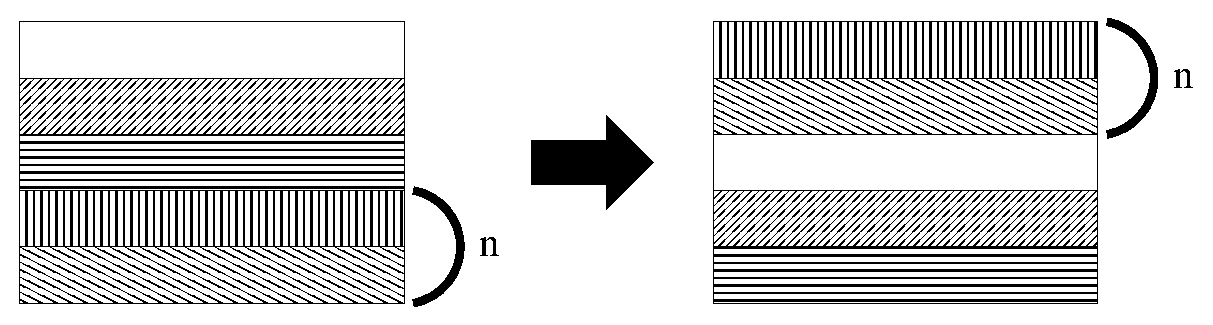
\includegraphics[width=12cm]{rotate-rows.eps}\\
\caption{Rotate-rows function.}
\end{figure}
\end{center}

\vspace*{-5mm}

%---------------------------------------------------------------------------%
% 066
\index{rotate\_cols!( int n )} 
\setNormalInstance
\printMethodWithOneParam
{array$<$ T $>$}
{rotate\_cols}
{int}
{n}
{The number of columns you want to put first ( See above ).}
{Changes the order of rows.}
{The array ( result ).}
{None.}
%---------------------------------------------------------------------------%

\clearpage

\subsection{Generating Methods}

%---------------------------------------------------------------------------%
% 068
\index{clone!( )} 
\setConstInstance
\printEmptyMethodReturn
{arraybase*}
{clone}
{Returns a copy of the current array.}
{A copy of the current array.}
%---------------------------------------------------------------------------%

%---------------------------------------------------------------------------%
% 069
\index{empty!( )} 
\setConstInstance
\printEmptyMethodReturn
{arraybase*}
{empty}
{Returns a new empty array.}
{A new empty array.}
%---------------------------------------------------------------------------%

\vspace*{10mm}

\subsection{Dummy Operators}

%---------------------------------------------------------------------------%
% 070
\index{operator ==!( const array$<$ T $>$\& )} 
\setConstInstance
\printMethodWithOneParam
{bool}
{operator ==}
{const array$<$ T $>$\&}
{}
{}
{The dummy operator.}
{False.}
{None.}
%---------------------------------------------------------------------------%

%---------------------------------------------------------------------------%
% 071
\index{operator $\mid$!( const array$<$ T $>$\& )} 
\setConstInstance
\printMethodWithOneParam
{bool}
{operator !=}
{const array$<$ T $>$\&}
{}
{}
{The dummy operator.}
{False.}
{None.}
%---------------------------------------------------------------------------%

\clearpage

%---------------------------------------------------------------------------%
% 072
\index{operator $<$!( const array$<$ T $>$\& )} 
\setConstInstance
\printMethodWithOneParam
{bool}
{operator $<$}
{const array$<$ T $>$\&}
{}
{}
{The dummy operator.}
{False.}
{None.}
%---------------------------------------------------------------------------%

%---------------------------------------------------------------------------%
% 073
\index{operator $>$!( const array$<$ T $>$\& )} 
\setConstInstance
\printMethodWithOneParam
{bool}
{operator $>$}
{const array$<$ T $>$\&}
{}
{}
{The dummy operator.}
{False.}
{None.}
%---------------------------------------------------------------------------%

\clearpage

\section{Private Methods}

\vspace*{10mm}

\subsection{Methods for resizing}

%---------------------------------------------------------------------------%
% 074
\index{resize\_i!( unsigned* \_d, unsigned \_nd, bool copy )}
\setNormalInstance
\setCorrectWidthThree{8pt}
\setParamOne{\_d}{unsigned*}{The pointer to the the dimension array.} 
\setParamTwo{\_nd}{unsigned}{The number of dimensions.}
\setParamThree{copy}{bool}{The flag of copy.}
\printMethodWithParamsSaved
{void}
{None.}
{resize\_i}
{Resizes the array.}
{None.}
\setCorrectWidthThree{4pt}
%---------------------------------------------------------------------------%

%---------------------------------------------------------------------------%
% 075
\index{array!( unsigned* \_d, T* \_e, unsigned \_nd, unsigned \_ne,
bool \_stat )}
\setNormalInstance
\setCorrectWidthThree{8pt}
\setParamOne{\_d}{unsigned*}{The pointer to the dimension array.} 
\setParamTwo{\_e}{T*}{The pointer to the element array.}
\setParamThree{\_nd}{unsigned}{The number of dimensions.}
\setParamFour{\_ne}{unsigned}{The number of elements.}
\setParamFive{\_stat}{bool}{The flag which signals whether object is a
static ref.}
\printMethodWithParamsSaved
{}
{None.}
{array}
{Copys data of array in the array ``{\em this}''.}
{None.}
\setCorrectWidthThree{4pt}
%---------------------------------------------------------------------------%

\clearpage

\section{Input and Output Methods}

%---------------------------------------------------------------------------%
% 070
\index{readFrom!( std::istream\& is )} 
\setNormalInstance
\printMethodWithOneParam
{void}
{readFrom}
{std::istream\&}
{is}
{Input stream.}
{Reads the array.}
{None.}
{None.}
%---------------------------------------------------------------------------%

%---------------------------------------------------------------------------%
% 071
\index{writeTo!( std::ostream\& os )} 
\setConstInstance
\printMethodWithOneParam
{void}
{writeTo}
{std::ostream\&}
{os}
{Output stream.}
{Writes the current array.}
{None.}
{None.}
%---------------------------------------------------------------------------%



